% !TEX root = ../oddp.tex

\subsection{From $\Omega_*(r)$ to the minimal resolution}\label{ss:mapf} The \emph{pivotal piece} of a pieced word $A_0\barra \ldots\barra A_k$ is the leftmost piece $A_j$ such that $A_{j+1}*\ldots*A_k$ has augmented dimension smaller than $r$.

\begin{example}
	If $r=5$, the pivotal piece of the pieced word $A=01|24|013|12|4$ is $A_1 = 013$, while $A_2 = 12|4$ and $\hat{A} = 01|24$. If $r=3$, the pivotal piece of the pieced word $01|20|1|02|1|20|12$ is $20$, while $A_2 = 12$ and $\hat{A} = 01|20|1|02|1$. 
\end{example}


The join homomorphism $\chains_*(\asimplex^{r-1}\join \asimplex^{r-1})\to \chains_*(\asimplex^{r-1})$ induces an endomorphism
\[
\kappa\colon \Omega_*(r)^0\lra \Omega_*(r)^0 
\]
that sends a pieced word $A_0\barra \ldots\barra A_k$ with pivotal piece $A_j$ to the pieced word $(-1)^{\lambda(A_{j+1},\ldots,A_k)}A_0\barra \ldots\barra A_j\barra A_{j+1}\join\ldots\join A_k$, where the sign is that of the permutation that orders the entries of $A_{j+1},\ldots,A_k$.

The cyclic group $\Cyc_r$ acts on $\partial \asimplex^{r-1}$ by permuting its vertices forwards. Let $\sigma$ be the top simplex of $\asimplex^{r-1}$ and define
\begin{align*}
	\iota_1\colon \chains_k(\sus{r-1}\partial \simplex^{r-1})&\lra \chains_{k}(\partial\simplex^{r-1})\otimes \chains_{r-1}(\partial\simplex^{r-1})\\
	\iota_2\colon \chains_k(\sus{r-1}\partial \simplex^{r-1})&\lra \chains_{r-1}(\partial\simplex^{r-1})\otimes \chains_{k}(\partial\simplex^{r-1})
\end{align*}
be the $\Cyc_r$-equivariant chain homomorphisms given by
\begin{align*}
	\iota_1(\tau) &= (-1)^{|\tau|}\tau\otimes \partial \sigma &
	\iota_2(\tau) &= \partial \sigma\otimes \tau
\end{align*}
Let $f\colon \chains_*(\partial\simplex^{r-1})\otimes\chains_*(\partial\simplex^{r-1})\to \chains_*(\sus{r-1}\partial\asimplex^{r-1})$ be a $\Cyc_r$-equivariant chain homomorphism such that
\renewcommand{\theenumi}{\roman{enumi}}
\begin{enumerate}
	\item\label{cond:1} $f\circ \iota_1 = \Id$
	\item\label{cond:2} $f\circ \iota_2 = \rho$.
	\item\label{cond:3} if $\tau_1\otimes\tau_2$ has degree $r$, then $ \partial f(\tau_1\otimes\tau_2) =
	\begin{cases}
	\pm\emptyset & \text{if $\tau_1* \tau_2$ is non-degenerate} \\
	0 & \text{otherwise},
	\end{cases}$
 where the last sign is the sign of the permutation that orders $\tau_1*\tau_2$.
\end{enumerate}

\begin{remark}
	Condition \eqref{cond:3} is implied by the following condition:
    \begin{itemize}
        \item[(iii')] If $\tau_1\otimes\tau_2$ has degree $r$, then $f(\tau_1\otimes \tau_2)$ is $\pm v$ for some vertex of $\asimplex^{r-1}$ if $\tau_1* \tau_2$ is non-degenerate and $0$ otherwise. The sign is that of the permutation that orders $\tau_1*\tau_2$.
    \end{itemize}
    \footnote{\federico{ 
    Condition \eqref{cond:3} is equivalent to the following condition:
    \begin{itemize}
    \item[(iii'')]if $\tau_1\otimes\tau_2$ has degree $r-1$, then $ f(\tau_1\otimes\tau_2) =
	\begin{cases}
	\pm \emptyset & \text{if $\tau_1* \tau_2$ is non-degenerate} \\
	0 & \text{otherwise},
    \end{cases}$
    where the sign is the one of the permutation that orders $a*\tau_1*\tau_2$, where $a$ is the only vertex such that $a*\tau_1*\tau_2$ is non-degenerate.
    \end{itemize}}}
\end{remark}




\begin{theorem} Each homomorphism $f$ satisfying Condition \eqref{cond:3} as above yields a chain endomorphism
\[
    S\colon \Omega_*(r)^{\nf}\lra \sus{r-1}\Omega_*(r)^{\nf}
\]
that sends a pieced word $A = A_0\barra \ldots\barra A_k$ with pivotal piece $A_j$ to the pieced word $ A_0\barra \ldots\barra f(A_j\otimes \kappa(A_{j+1}\barra \ldots\barra A_k))$.
\end{theorem}
\begin{proof}
    Replacing the word $A$ by $\kappa(A)$, we may assume that $A_{j+1} = A_k$. Let $\bar{A} = A_0\barra \ldots\barra A_{j-1}$ and let $\ell$ be the degree of $\bar{A}$ (i.e., the number of entries of $A$). Then %and recall that $\partial A = \sum_{i} (-1)^{i}d_iA$, where $d_i$ removes the $i$-th entry of $A$. Then
	\begin{equation}\label{eq:931}
		\partial S(A) = \partial \bar{A}\mid f(A_{j}\otimes A_{j+1}) + (-1)^{\ell}\bar{A}\barra \partial f(A_{j}\otimes A_{j+1}).
	\end{equation}
	We distinguish two cases: if $A_j$ has length at least $2$,
	\[S(\partial A) = \partial \bar{A}\barra f(A_j\otimes A_{j+1}) + (-1)^{\ell}\bar{A}\barra f(\partial (A_j\otimes A_{j+1})),\]
	which equals the previous sum. If $A_j$ has length $1$, let $\check{A} = A_0\mid \ldots\mid A_{j-2}$. Then
	\begin{equation}\label{eq:933}
		S(\partial A) = \partial \bar{A}\barra f(A_j\otimes A_{j+1}) + (-1)^\ell \check{A}\barra f(A_{j-1}\otimes \partial(A_j*A_{j+1})).
	\end{equation}
	Let $\pm$ be the sign of the permutation that orders $A_1*A_2$. By condition \eqref{cond:3}, the last summand of \eqref{eq:931} is zero or $\pm(-1)^\ell\bar{A}$ depending on whether $A_j*A_{j+1}$ is degenerate or not, which by condition \eqref{cond:1} is equivalent to $f(A_{j-1},\partial(A_j*A_{j+1}))$ being $0$ or $\pm(-1)^{\ell}A_{j-1}$, and therefore equivalent to the last summand of \eqref{eq:933} being zero or $\pm(-1)^{\ell}\bar{A}$.
\end{proof}

%The inclusion of the augmented $1$-skeleton of $\asimplex^{r-1}$ in $\asimplex^{r-1}$ induces an inclusion $\chains_*(\EC_r)\to \Omega_*(r)^0$ that sends a word to that same word with all pieces of length $1$. 

\begin{definition}
	Define a homomorphism $\Psi\colon \Omega_*(r)^{\nf}\to \rW_*(r)$ recursively as
	\[\Psiom_q(A) = \begin{cases} \Phi_q(\kappa(A)) & \text{if $q\leq r-1$} \\
		\frac{1}{\tilde{r}!}\theta_{1-r}\Psiom_{q-r+1}S(A) & \text{if $q\geq r$.}\end{cases}\]
\end{definition}

\begin{lemma}
	$\Psiom$ is a chain homomorphism. %$\Psiom\partial = \partial\Psiom$
\end{lemma}
\begin{proof}
The first expression is already a chain homomorphism. To check that it is also a homomorphism in degree $r$, we distinguish two cases: if $\Psiom(A) = 0$, then $A$ has repeated entries. If it has one repeated entry, then the image by $\Psiom$ of its boundary has two canceling terms, while if it has more repeated entries, it is zero on the nose. If $\Psiom(A)\neq 0$, then $A$ has no repetitions, and we can assume without loss of generality that $A=(0,1,\ldots,r)$ therefore $\Psiom(d_iA) = (-1)^{i+2}\rho^{i+1} e_{r-1}$. Hence, $\Psiom(\partial A) = \sum (-1)^i\Psiom(d_iA) = \sum \rho^{i+1} e_{r-1} = Ne_{r-1} = \partial \Psi_r(A)$. The second expression is then proven to be a chain homomorphism by induction. 
%	We already know that it is a chain homomorphism in degrees $*\leq r-2$. The verification in higher degrees follows from Lemma \ref{lemma:pieced_suspension} and induction. 
 %(for clarity, we omit the factor $\frac{1}{\tilde{r}!}$):
%	\begin{align*}
%		\Psiom_{q-1}\partial(A) &= {\textstyle\frac{1}{\tilde{r}!}}\theta_{1-r}\Psiom_{q-r}S\partial(A) = {\textstyle\frac{1}{\tilde{r}!}} \theta_{1-r}\Psiom_{q-r}\partial S(A) = \\
%		&={\textstyle\frac{1}{\tilde{r}!}}\theta_{1-r}\partial\Psiom_{q-r+1}S(A) = {\textstyle\frac{1}{\tilde{r}!}}\partial\theta_{1-r}\Psiom_{q-r+1}S(A) = \partial \Psiom_{q}(A).
%	\end{align*}
%	Finally, recall that the map $\Psi_{r-2}$ of the previous section has a factor of $\frac{1}{\tilde{r}!}$ and consists on all permutations of $\{0,1,\ldots,r-1\}$, hence one deduces from \eqref{cond:3} that $\frac{1}{\tilde{r}!}\theta_{r-1}\Psiom_{-1}S(A) = \Psiom_{r-2}(A)$, hence both definitions coincide at their common case.
\end{proof}

%\begin{lemma} $\bar{\Psi}_{q-1}((\partial A)^{nf}) = \partial\bar{\Psi}_{q-r}\DDD(A)$ if $A$ has a full piece.
%\end{lemma}
%\begin{proof}
%\begin{itemize}
%\item if the full piece is to the left of $w_1$ \fcnote{doublecheck this, if it is exactly to the left an additional argument may be needed}, then $S\partial(A) = \partial S(A)$.
%\item if the full piece is to the right of $w_1$, then let $A_3$ be that full piece, and assume, without loss of generality that is the last piece. Then
%\[\partial S(A) = \partial \bar{A}*f(A_1,A_2)*A_3 + \bar{A}*\partial f(A_1,A_2)*A_3 + \bar{A}*f(A_1,A_2)*\partial A_3\]
%\[S\partial(A) = \partial \bar{A}*f(A_1,A_2)*A_3 + \bar{A}*\partial f(A_1,A_2)*A_3 + \bar{A}*A_1*f(A_2,\partial A_3)\]
%We need to check that the value of $\Psiom$ in the last term coincides. If $q-r+1\geq r-2$, then we have that
%\[\Psiom(\bar{A}*f(A_1,A_2)*\partial A_3) = \PsiomS(\bar{A}*f(A_1,A_2)*\partial A_3) = \Psiom(\bar{A}*f(f(A_1,A_2),\partial A_3)\]
%\[\Psiom(\bar{A}*A_1*f(A_2,\partial A_3)) = \PsiomS(\bar{A}*A_1*f(A_2,\partial A_3)) = \Psiom(\bar{A}*f(A_1*f(A_2,\partial A_3))\]
%and both terms equal $f(A_1,A_2)$.
%\end{itemize}
%
%\end{proof}

\begin{lemma} If the map $f$ satisfies conditions \eqref{cond:1} and \eqref{cond:2}, then
\[
    \tilde{r}!\Psiom_{q-1}((\partial^{\f} A)) = (-1)^{q-r}\theta_{1-r}\circ \Psiom_{q-r}\circ\DDD(A).
\]
%and there are $\ell$ elements to the left of the full piece.
\end{lemma}

\begin{proof}
	We will prove it by induction on the position of the full piece from the right.If $A$ has no full pieces, then both sides vanish. Since $A$ has one full piece, $q\geq r-1$. We distinguish three cases:

	If the full piece is the last piece, write $A=\bar{A}*A_1*A_2$ with $A_2 = \sigma$ the full piece and $A_1$ the penultimate piece, and let $\ell = q-r$ be the length of $\bar{A}*A_1$. Then by Condition \eqref{cond:1}: 
	\begin{align*}
	    \tilde{r}!\Psiom_{q-1}((\partial A)^{nf}) &=
		\theta_{1-r} \Psiom_{q-r}(S(\partial(A)^{nf})) \\
		&= (-1)^{\ell} \theta_{1-r}\Psiom_{q-r}(S(\bar{A}*A_1*\partial A_2)) \\
		&= (-1)^{\ell} \theta_{1-r}\Psiom_{q-r}(\bar{A}*f(A_1\otimes \partial \sigma)) \\
		&= (-1)^{\ell} \theta_{1-r}\Psiom_{q-r}(\bar{A}*A_1) \\
		&= (-1)^{q-r}\theta_{1-r}\Psiom_{q-r}\DDD(A).
	\end{align*}
	If the full piece is the penultimate piece, write $A=\bar{A}*A_1*A_2$ with $A_1$ the full piece and $\ell$ for the length of $\bar{A}$. Then by Condition \eqref{cond:2}:
	\begin{align*}
	    \tilde{r}!\Psiom_{q-1}((\partial A)^{nf}) &=
        \theta_{1-r}\Psiom_{q-r}(S(\partial(A)^{nf})) \\
        &= (-1)^{\ell}\theta_{1-r}\Psiom_{q-r}(S(\bar{A}*\partial A_1* A_2)) \\
		&= (-1)^{\ell} \Psiom_{q-r}(\bar{A}*f(\partial A_1\otimes A_2)) \\
		&= (-1)^{\ell} \theta_{1-r}\Psiom_{q-r}(\bar{A}*\rho(A_2)) \\
		&= (-1)^{q-r}\theta_{1-r}\Psiom_{q-r}\DDD(A).
	\end{align*}
	   Otherwise, $q\geq 2r$, and we reason by induction as follows: %write $A=\bar{A}_1*\bar{A}*\bar{A}_2*A_1*A_2$ with $A_1$ the piece that contains the last pivot and $A_2$ the word to the right of $A_1$. Assume by induction that the lemma holds for words of smaller length. Then
    \begin{align*}
        \tilde{r}!\Psiom_{q-1}((\partial A)^{nf}) 
        &= \tilde{r}!\theta_{1-r} \Psiom_{q-r}(S(\partial A)^{nf}) \\
        &= \tilde{r}!\theta_{1-r} \Psiom_{q-r}((\partial SA)^{nf}) \\
        &= (-1)^{q-r}\theta_{1-r}\theta_{1-r} \Psiom_{q-2r+1}(\DDD (SA)) \\
        &= (-1)^{q-r}\theta_{1-r}\theta_{1-r} \Psiom_{q-2r+1}(S(\DDD A)) \\
        &= (-1)^{q-r}\theta_{1-r} \Psiom_{q-r}(\DDD A)\qedhere
    \end{align*}
\end{proof}





 

\subsection{Barycentric subdivisions and the map $f$} Recall that the barycentric subdivision $\sd \simplex^n$ of the geometric simplex $\simplex^n$ is the ordered simplicial complex that has one vertex for each non-empty face of $\simplex^n$ and one face $(\sigma_0,\ldots,\sigma_k)$ of dimension $k$ for every ascending chain $\sigma_0\subset \sigma_1\subset\ldots \subset \sigma_k$ of simplices of $\simplex^n$. We will denote the face $(\sigma_0,\ldots,\sigma_k)$ as $(a_0|a_1|\ldots|a_k)$, where $a_i = \sigma_i\smallsetminus \sigma_{i-1}$. With this notation, the differential on $\chains_*(\simplex^n)$ becomes
\[
\partial(a_0|a_1|\ldots|a_k) = \sum_{i=0}^{k-1} (-1)^i(a_0|\ldots|a_i*a_i+1|\ldots |a_k|) + (-1)^k (a_0|\ldots|a_{k-1}).
\]
The \emph{pair barycentric subdivision}\footnote{Here we are flipping the order of $a,b$ to fit the convention of the rest of the paper, in which we are writing cochains on the left} $\Psd \simplex^n$ of $\simplex^n$ is a cubulation of $\simplex^n$ with the same vertices as $\sd \simplex^n$ and one face for each pair $(b,a)$ of faces of $\simplex^n$ such that $b\subset a$. Geometrically, that face is the union of all the faces of the barycentric subdivision that correspond to ascending chains $b\subset \sigma_0\subset \ldots\subset \sigma_k\subset a$. Interpreting $b$ as a dual cochain, its chain complex $\chains_*(\Psd \simplex^n)$ is isomorphic to the tensor product $\chains^*(\simplex^n)\otimes \chains_*(\simplex^n)$ modulo the pairs $b\otimes a$ such that the support of $b$ is not contained in $a$. It has the following differential:
\[\partial(b\otimes a) = (-1)^{|b|}(\delta b\otimes a + b\otimes \partial a)\]
%\[\partial(a\otimes b) = \partial a + (-1)^{|a|-|b|} \delta b\]
There are chain homomorphisms
\[
\xymatrix{
&\chains_*(\simplex^n)\otimes \chains_*(\simplex^n)\ar[d]^h& \\
\chains_*(\simplex^n)\ar[r]^{s_*^{\simplex}}\ar@/_2.0pc/[rr]^{s_*} & \chains_*(\Psd \simplex^n)\ar[r]^{s^{\Psd}} & \chains_*(\sd\simplex^n) 
}
\]
defined as follows \cite[\P 1.12]{Rounds2010}):
\[
    s_*([a_0,\ldots,a_k]) = \sum_{\sigma\in \Sigma_{k+1}} (-1)^{\sgn(\sigma)}(a_{\sigma(0)}|a_{\sigma(1)}|\ldots|a_{\sigma(k)}).
\]
If $b\subset a$ and $b\smallsetminus a = (c_0,\ldots,c_{k})$,
\[
s_*^{\Psd}(b\otimes a) = \sum_{\sigma\in \Sigma_{k+1}} (-1)^{\sgn(\sigma)} (b|c_{\sigma(0)}|c_{\sigma(1)}|\ldots|c_{\sigma(k)})
\]
\[
s_*^{\simplex}([a_0,\ldots,a_k]) = \sum_{j=0}^k (-1)^j[a_j]\otimes [a_0,\ldots,a_k]
\]
\[
h( b\otimes a) = (-1)^{n+1}\alex(b)\otimes a
\]

The Alexander duality homomorphism induces simplicial endomorphisms of the barycentric and the pair subdivision
\begin{align*}
\alex\colon \sd \simplex^n&\lra \sd \simplex^n,
&
\alex\colon \Psd \simplex^n&\lra \Psd \simplex^n.
\end{align*}
The first one sends an ascending chain of simplices $(\sigma_0,\ldots,\sigma_{k-1})$ to the asceding chain of their complementary simplices $(-1)^{k+1}(\sigma_{k-1}^c,\ldots,\sigma_0^c)$. The second one sends $b\otimes a$ to $(-1)^{|a||b|}\Lambda(a)\otimes \Lambda(b)$. In addition we have the twist
\[\mathrm{twist}\colon \uchains_*(\asimplex^n)\otimes \uchains_*(\asimplex^n)\lra \uchains_*(\asimplex^n)\otimes \uchains_*(\asimplex^n)\]
that sends $a\otimes b$ to $(-1)^{|a||b|} b\otimes a$.
\begin{definition}
    An \emph{assemblage map} is a simplicial map $g\colon \simplex^n\to \sd \simplex^n$ such that the composition $g_*\circ s_*$ is the identity.
\end{definition}
\begin{definition}
    A \emph{$(n+1)$-cyclic assemblage map} is an assemblage map that is cyclic with respect to the forward action of the cyclic group $C_{n+1}$ on $\simplex^n$.
\end{definition}
\begin{definition}
    A \emph{$(n+1)$-cyclic assemblage map with duality} is a cyclic assemblage map $g$ such that the composition
    \[\sd \simplex^n \overset{\alex}{\lra} \sd \simplex^n \overset{g}{\lra} \simplex^n\overset{\rho}{\lra} \simplex^n \]
    is also an assemblage map.
\end{definition}

\begin{proposition} Let $r$ be odd.
    If $g$ is an $r$-cyclic assemblage map with duality, then the composition $f = g_*\circ s_*^{\Psd}\circ h_*\circ \mathrm{twist}$ satisfies the conditions of Section \ref{ss:mapf}.
\end{proposition}
\begin{proof}
For condition \ref{cond:1},
\begin{align*}
g_*\circ s_*^{\Psd}\circ h \circ \mathrm{twist}(\tau\otimes \partial\sigma)
&= g_*\circ s_*^{\Psd}\circ h (\partial\sigma\otimes \tau)\\ 
&= g_*\circ s_*^{\Psd}(\sum \pm (v\otimes\tau)) \\
&= g_*\circ s_*^{\Psd}\circ s_*^{\simplex}(\tau) \\
&= \tau.
\end{align*}
For condition \ref{cond:2}, notice that the following diagram commutes:
\[\xymatrix{
C_*(\partial \simplex^n*\partial\simplex^n)\ar[r]^h\ar[d]^{\text{twist}} &C_*(\Psd \partial \simplex^n) \ar[r]^{s_*^{\Psd}}\ar[d]^{\alex}& C_*(\sd \partial \simplex^n)\ar[d]^{\alex}\\
C_*(\partial \simplex^n*\partial\simplex^n)\ar[r]^h &C_*(\Psd \partial \simplex^n) \ar[r]^{s_*^{\Psd}}& C_*(\sd \partial \simplex^n).
}\]
and therefore, using Condition \eqref{cond:1},
\[
g_*\circ s_*^{\Psd}\circ h \circ \mathrm{twist}(\partial\sigma\otimes \tau) = g_*\circ \Lambda\circ s_*^{\Psd}\circ h \circ \mathrm{twist}(\tau\otimes \partial\sigma) = \rho^{-1}(\tau).
\]
Finally, for Condition \ref{cond:3} notice that, if $(\tau_1,\tau_2)$ has degree $r$, and $\tau_1*\tau_2$ is non-degenerate, then $\tau_2 = \check{\tau}$ and
\[
h\circ\twist(\tau_1,\tau_2) = (-1)^{|\tau_1||\tau_2|}(-1)^{\lambda(\tau_2)}\tau_1\otimes \tau_1
\]
Finally, notice that $g_*\circ s_*^{\Psd}(\tau_1\otimes \tau_1)$ is zero or a vertex if $\tau_1*\tau_2$ is degenerate or not, and that the sign obtained above is the sign that orders $\tau_1*\tau_2$.
\end{proof}



%\begin{proposition} If $f\colon C_*(\partial \simplex^n)\otimes C_*(\partial \simplex^n)\lra C_*(\Sigma^n\partial \simplex^n)$ is a homomorphism satisfying the conditions, then $f$ factors as
%\[f = g\circ s_*^{\Psd}\circ m\]
%for some cyclic assemblage map with duality $g$.
%\end{proposition}
%\begin{proof}
%The map $m$ is universal among maps that annihilate pairs of faces that do not span the whole simplex, therefore $f$ does factor %through $m$. Secondly, any map from the pair subdivision of $\partial \simplex^n$ to a simplicial complex factors through the barycentric subdivision. Condition \eqref{cond:3} guarantees that the resulting map $g$ is simplicial.The proof on the previous proposition can be followed to show that Conditions \eqref{cond:1} and \eqref{cond:2} for $f$ translate into $g$ being a assemblage map with duality.
%\end{proof}
%}

Observe that $\Cyc_r$ acts freely on the vertices of $\partial \simplex^{r-1}$, but it only acts freely on the vertices of $\partial \sd\simplex^{r-1}$ if $r$ is prime. Therefore $r$-cyclic assemblage maps only exist if $r$ is prime. On the other hand, the following lemma, pointed to us by Martin Palmer, assures the existece of such maps when $r$ is prime.
\begin{lemma} An $r$-cyclic assemblage map with duality is the same as a  $\Cyc_r$-equivariant choice of an element $x_\tau$ in each proper subset $\tau$ of $\{0,1,\ldots,n\}$ such that its cyclic predecessor $x_\tau-1$ is not in $\tau$.
\end{lemma}
\begin{example}
    If $r=3$, the only assemblage map with duality comes from the choice
    \begin{align*}
        [0]&\mapsto 0 & [0,1]&\mapsto [0]
    \end{align*}
\end{example}
\begin{example}
    If $r=5$, there are four assemblage maps with duality corresponding to the following choices:
    \begin{align*}
        [0]&\mapsto 0 & [0,1]&\mapsto 0 & [0,2]&\mapsto 0 & [0,1,2]&\mapsto 0 & [0,1,3] & \mapsto 0 & [0,1,2,3] & \mapsto 0 \\
        [0]&\mapsto 0 & [0,1]&\mapsto 0 & [0,2]&\mapsto 2 & [0,1,2]&\mapsto 0 & [0,1,3] & \mapsto 0 & [0,1,2,3] & \mapsto 0 \\
        [0]&\mapsto 0 & [0,1]&\mapsto 0 & [0,2]&\mapsto 0 & [0,1,2]&\mapsto 0 & [0,1,3] & \mapsto 3 & [0,1,2,3] & \mapsto 0 \\
        [0]&\mapsto 0 & [0,1]&\mapsto 0 & [0,2]&\mapsto 2 & [0,1,2]&\mapsto 0 & [0,1,3] & \mapsto 3 & [0,1,2,3] & \mapsto 0
    \end{align*}
\end{example}
If $r=7$ there are several thousands of assemblage maps with duality. 
\begin{figure}
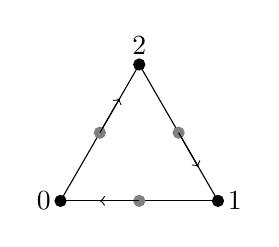
\begin{tikzpicture}
    \draw (0,1.732) -- (1,0);
    \draw (-1,0) -- (1,0);
    \draw (-1,0) -- (0,1.732);
    \filldraw [gray] (-.5,.866) circle (2pt);
    \filldraw [gray] (.5,.866) circle (2pt);
    \filldraw [gray] (0,0) circle (2pt);
    \filldraw [black] (0,1.732) circle (2pt)  node[anchor=south]{2};
    \filldraw [black] (1,0) circle (2pt) node[anchor=west]{1};
    \filldraw [black] (-1,0) circle (2pt) node[anchor=east]{0};
    \draw[->] (0,0) -- (-.5,0);
    \draw[->] (-.5,.866) -- (-.25,1.299);
    \draw[->] (.5,.866) -- (.75,.433);
\end{tikzpicture}
\caption{The cyclic subdivision map for $\partial \simplex^2$.}
\end{figure}

\begin{figure}
\begin{tikzpicture}[line join = round, line cap = round]
\pgfmathsetmacro{\factor}{1/sqrt(2)};
\coordinate [label=left:A] (A) at (-2,0,0);
\coordinate [label=below:B] (B) at (.4,-1,0);
\coordinate [label=right:2] (C) at (2,0,0);
\coordinate [label=above:3] (D) at (0,2.8,.2);

path (B) -- (C) node[midway] (BC) {BC}

\coordinate (AB) at ($ (A)!0.5!(C) $); % Anibal: I modified this line to get rid of an error
\coordinate (AC) at (0,0,0);
\coordinate (AD) at (2,0,0);
\coordinate (D) at (0,2.8,.2);

%\draw[->] (0,0) -- (3,0,0) node[right] {$x$};
%\draw[->] (0,0) -- (0,3,0) node[above] {$y$};
%\draw[->] (0,0) -- (0,0,3) node[below left] {$z$};
\foreach \i in {A,B,C,D}
    \draw[dashed] (\i) -- (AB);
\draw[-, fill=red!30, opacity=.5] (A)--(D)--(B)--cycle;
\draw[-, fill=green!30, opacity=.5] (A) --(D)--(C)--cycle;
\draw[-, fill=purple!30, opacity=.5] (B)--(D)--(C)--cycle;
\end{tikzpicture}
    \caption{The cyclic subdivision map for $\partial \simplex^4$ on the face $[0,1,2,3]$ (the other faces are in the $C_r$-orbit of this face). \federico{to be discarded if it is too complicated}}
    \label{fig:my_label}
\end{figure}
\begin{example}\label{ex:107}
    Let us find the image of $01|20|1|02|1|20|12$ for $r=3$ under $\Psi$:
    \begin{align*}
        \Psi_{12}(01|20|1|02|1|20|12) &= \theta_2\Psi_{10}(01|20|1|02|1|f([20]\otimes[12])) = \theta_2\Psi_{10}(01|20|1|02|1|20)
        \\ &= \theta_4\Psi_8(01|20|1|02|f([1]\otimes [20])) = \theta_4\Psi_8(01|20|1|02|1)
        \\ &= \theta_6\Psi_6(01|20|1|f([02]\otimes [1])) = \theta_6\Psi_6(01|20|1|2)
        \\ &= \theta_8\Psi_4(01|f([20]\otimes [12])) = \theta_8\Psi_4(01|20)
        \\ &= \theta_{10}\Psi_2(f([01]\otimes [20])) = \theta_{10}\Psi_2(01)
        \\ &= e_{12}
    \end{align*}
\end{example}


